\begin{figure}[h]
    \centering
    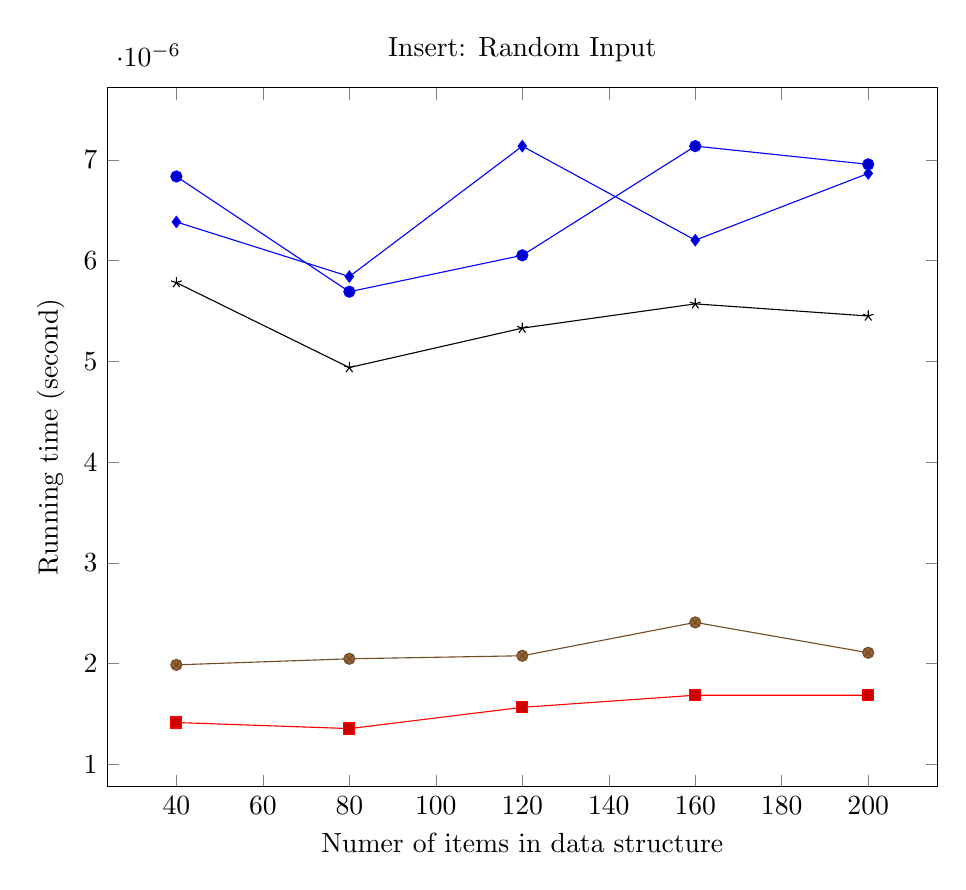
\begin{tikzpicture}
        \begin{axis}[
            xlabel={Numer of items in data structure},
            ylabel={Running time (second)},
            title={Insert: Random Input},
            width=\textwidth
        ]
		\addplot coordinates {
			(40, 6.836680144317598e-06)
			(80, 5.692213864350038e-06)
			(120, 6.053624268886892e-06)
			(160, 7.1378554810763715e-06)
			(200, 6.957150278807944e-06)
		};
		\addplot coordinates {
			(40, 1.4155240826596582e-06)
			(80, 1.355289015236849e-06)
			(120, 1.566111751216681e-06)
			(160, 1.6865818860622995e-06)
			(200, 1.686581885707028e-06)
		};
		\addplot coordinates {
			(40, 1.9877572224658024e-06)
			(80, 2.047992290243883e-06)
			(120, 2.0781098236000163e-06)
			(160, 2.4094026940701953e-06)
			(200, 2.1082273573114206e-06)
		};
		\addplot coordinates {
			(40, 5.782566465484251e-06)
			(80, 4.939275522630737e-06)
			(120, 5.330803460523726e-06)
			(160, 5.57174372985969e-06)
			(200, 5.4512735950140724e-06)
		};
		\addplot coordinates {
			(40, 6.3849171390018e-06)
			(80, 5.842801532907061e-06)
			(120, 7.1378554810763715e-06)
			(160, 6.204211937088644e-06)
			(200, 6.866797678029002e-06)
		};
        \legend{}
        \end{axis}
    \end{tikzpicture}
    \caption{Average of 0 operations, benchmarked every 0, starting at 0.}
\end{figure}